\documentclass[conference]{IEEEtran}
\usepackage{cite}
\usepackage{amsmath,amssymb}
\usepackage{graphicx}
\usepackage{booktabs,array}
\usepackage{balance}
\usepackage[hidelinks]{hyperref}
\emergencystretch=1em
\graphicspath{{../figures/}}

\begin{document}
\title{DentDES: A Factorial Discrete-Event Evaluation of Appointment Spacing and Readiness-Aware Dispatch in Dental Clinics}
\ifdefined\NamedVersion
\author{\IEEEauthorblockN{Fatemeh ASTARAKI}
\IEEEauthorblockA{\textit{Ankara Medipol University}\\
Ankara, T\"{u}rkiye \\
fatemeh.astaraki@std.ankaramedipol.edu.tr\\
ORCID: 0009-0005-3004-2206}
\and
\IEEEauthorblockN{Mehmet Ali Akyol}
\IEEEauthorblockA{\textit{Beko; Ankara Medipol University}\\
Ankara, T\"{u}rkiye\\
mehmetali.akyol@beko.com\\
mehmet.akyol@ankaramedipol.edu.tr\\
ORCID: 0000-0001-8196-946X}
}


\else
\author{}
\fi
\maketitle

\begin{abstract}
Patients can be ready for treatment while a chair is idle because the required instrument kit is still being reprocessed. We study whether appointment spacing or choosing another patient with a ready kit reduces this delay. DentDES models registration, treatment, chair turnover, and kit reprocessing in a synthetic discrete-event simulation. We compare four policy combinations at four demand levels and three kit capacities, using 50 paired replications of 30 independent clinic days. Every policy sees the same attendance and service inputs, and all attending patients eventually complete care. At the reference demand with two kits per procedure class, feasible-patient dispatch reduces mean arrival-to-treatment-start waiting from 127.94 to 92.96 minutes, a paired difference of $-34.99$ minutes (95\% confidence interval $[-35.90,-34.07]$). The appointment-spacing rule alone changes waiting by $+0.40$ minutes and adds little when combined with dispatch. The dispatch effect falls from 35.17 to 1.47 minutes when capacity rises from two to four kits per class. Overtime remains high in the constrained cases. These are conditional simulation results; clinic data and field testing are still needed before operational use.
\end{abstract}

\begin{IEEEkeywords}
dental operations, discrete-event simulation, appointment scheduling, instrument availability, resource coordination, paired experiments
\end{IEEEkeywords}

\section{Introduction}
Dental clinics coordinate staff, rooms, patients, and reusable instruments. Dental DES studies have examined resource utilization and waiting \cite{atalan2023}, and other work has combined treatment-duration prediction with simulation-based appointment scheduling \cite{chang2018}. Broader healthcare DES reviews show that most studies focus on time and efficiency, while relatively few report implementation after the modeling stage \cite{gunal2010,vazquez2021}. Appointment-scheduling reviews also emphasize arrival and service variability, provider preferences, and the information available to schedulers \cite{cayirli2003,gupta2008}. These findings leave a practical question for dental operations: if the first registered patient needs a kit that is unavailable, should another feasible patient start, and does appointment spacing change the answer?

The question links the appointment made in advance to the dispatch decision made during the clinic day. Under strict first-come-first-served (FCFS), a first patient can hold the queue while other resources sit idle. Starting a later feasible patient may reduce that blockage, although repeated bypasses can make the blocked patient's wait worse. A spacing rule changes arrival timing but does not change how quickly kits return. We therefore compare the rules with the same attendance and physical service inputs.

DentDES evaluates these decisions in an offline clinic model. It separates the effects of spacing and patient selection, tests their combination, and varies demand and kit capacity. The model treats chair cleaning and kit release as separate events, so it can distinguish queue blocking from delay caused by insufficient workload capacity. The inputs are synthetic; real-time sensing, learning, and clinical deployment are outside the scope of this study.

The contribution of this paper is a controlled, matched-input factorial evaluation of these two clinic policies. It quantifies when readiness-aware dispatch changes waiting under class-specific kit scarcity, tests whether the effect persists across demand and capacity levels, and reports the associated bypass and overtime tradeoffs. The study therefore contributes a bounded simulation comparison and an explicit evaluation protocol, rather than a claim of a deployed AI, IoT, or digital-twin system.

\section{Related Work and Research Position}
Atalan and Keskin use DES to estimate utilization and waiting in a dental clinic, comparing simulated activity with actual clinic counts \cite{atalan2023}. Chang and Chang evaluate individualized dental appointment scheduling with an artificial neural network and DES, including heterogeneous providers and patient pathways \cite{chang2018}. Kamali et al. model a dental clinic with additive manufacturing, inventory control, rest periods, and clinic--laboratory coordination \cite{kamali2022}. Together, these studies show that dental flow, scheduling, and inventory are established modeling settings.

Waiting and overtime have also been studied together outside dentistry. Gul et al. compare sequencing heuristics with a bi-criteria genetic algorithm for an outpatient procedure center \cite{gul2011}. Sterilization studies have modeled the processing service itself \cite{dimascolo2013}, while operating-room reviews cover capacity, sequencing, and resource allocation \cite{cardoen2010,guerriero2011}. Harris et al. connect operating-room and sterilization-processing simulation to block schedules and tray configurations \cite{harris2024}; Bos et al. combine sterilization-cycle simulation with tray-inventory optimization \cite{bos2026}. This study evaluates a dental queue policy that bounds patient overtaking, holds patient inputs constant across policies, and reports both capacity effects and the patients who wait longer after dispatch.

Queue fairness provides a related operations-research frame. Dynamic multipriority patient scheduling treats waiting-time targets as explicit constraints rather than relying only on FCFS order \cite{patrick2008}. Empirical hospital-flow analysis also documents overtaking and FCFS violations and discusses their implications for patient fairness \cite{armony2015}. Our bounded-bypass rule is a simpler operational safeguard: it permits a feasible patient to proceed while limiting repeated overtakes; it is not a priority optimization method or a fairness guarantee.

Healthcare digital-twin work sets a different evidential standard. Appuhamilage et al. implement a critical-care architecture and evaluate event collection and physical-to-digital synchronization \cite{appuhamilage2025}. Adjacent surgical settings also show that RFID can capture instrument state: Kranzfelder et al. detected tagged laparoscopic instruments in real time, and Hill et al. evaluated RFID-based measurement of intraoperative instrument use \cite{kranzfelder2013,hill2022}. These studies support the feasibility of a future resource-state feed, but they do not validate the synthetic state inputs used here. DentDES evaluates offline counterfactuals and does not make deployment claims. We also follow reporting guidance for healthcare DES by stating the assumptions, inputs, outcomes, and verification checks explicitly \cite{zhang2020}.


\section{Clinic Model and Policies}
\subsection{Scope and Physical Processes}
The model uses SimPy 4.1.2, a process-based DES framework \cite{simpy}. Figure~\ref{fig:model} shows patient flow and resource return. It represents four chairs, two interchangeable dentists, three interchangeable assistants, one front-desk worker, and one batch sterilizer. Each day starts with all kits available. Admissions occur during a 480-minute opening period, and the event queue then drains until patients, turnover tasks, and instrument cycles finish. Each day is an independent terminating experiment rather than one segment of a continuous calendar simulation.

Four procedure classes represent routine, restorative, impression, and complex appointments. Each patient needs one kit from the matching class. Kits can be exchanged within a class but not across classes. This abstraction gives the experiment class-specific resource scarcity; it is not a validated dental inventory. Consumables and replenishment are outside the model.

Patients register at the front desk and then join a queue for a clean chair, a dentist, an assistant, and the matching kit. The model acquires these resources together, so a patient cannot hold some of them while waiting for the rest. Treatment and documentation use all four. The dentist and assistant are released afterward, while checkout uses the front desk independently of chair turnover.

When an assistant becomes free, turnover takes priority over a new treatment. The assistant cleans the chair first and then prepares the used kit for reprocessing. The sterilizer starts a batch as soon as it is free and dirty kits are waiting, taking up to four of the oldest kits. The kits return together after the cycle. These rules and all physical durations are the same for every policy. Chair cleaning and kit reprocessing remain separate, so a chair can return before the previous patient's kit.

\begin{figure*}[t]
\centering
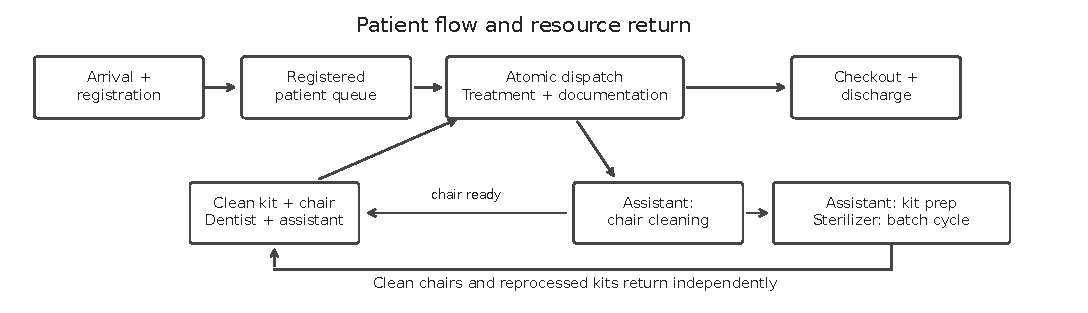
\includegraphics[width=.98\textwidth]{model_flow.pdf}
\caption{Implemented patient and resource flow. Treatment requires joint resource availability; chair cleaning, kit preparation, and batch reprocessing determine subsequent readiness. Patient checkout proceeds independently of turnover. Both policies use identical physical processes.}
\label{fig:model}
\end{figure*}

\subsection{Synthetic Inputs and Assumptions}
Table~\ref{tab:inputs} lists the synthetic assumptions. For each patient, the base treatment duration is first drawn from a normal distribution with a 30-minute mean multiplied by the procedure-class factor and an 8-minute SD, then clipped to 12--65 minutes. Independently, with probability 0.22, the model draws an exponential overrun with a 13-minute mean and adds it after clipping. No second upper clip is applied, so the realized duration can exceed 65 minutes only because of this overrun. These values are not fitted to clinic observations. The model draws patient inputs once before comparing policies. The scheduler sees request order and procedure class, but not future treatment duration, attendance, or resource availability.

Instrument preparation takes eight minutes. The synthetic batch cycle takes 29 minutes, including a 24-minute processing component and a five-minute release/drying proxy. These values define computational scenarios, not validated sterilizer settings. Dental sterilization monitoring must follow manufacturer-specified time, temperature, and pressure conditions \cite{cdc}; the model does not shorten a cycle.

\begin{table}[t]
\caption{Common Inputs and Experimental Factors}
\label{tab:inputs}
\centering\footnotesize
\begin{tabular}{@{}p{.40\linewidth}p{.55\linewidth}@{}}
\toprule
Quantity & Specification \\
\midrule
Requests/day & 22, 28, 34, 42 (0.8, 1.0, 1.2, 1.5$\times$) \\
Kits per class & 1, 2, 4; reference: 2 \\
Procedure probabilities & 0.52, 0.28, 0.13, 0.07 \\
Class multipliers $m_c$ & 0.82, 1.10, 1.00, 1.45 \\
No-show probability & 0.13, common across policies \\
Arrival deviation & Normal: mean 0, SD 6; bounds $\pm12$ min \\
Registration / checkout & Normal: mean 3, SD 0.8; minimum 1 min \\
Documentation & Normal: mean 8, SD 1.8; minimum 3 min \\
Chair cleaning & Normal: mean 9, SD 1.5; minimum 4 min \\
Kit preparation / cycle & 8 / 29 min, fixed \\
Replications & 50 blocks of 30 independent days \\
\bottomrule
\end{tabular}
\end{table}

\subsection{Appointment Spacing Factor S}
S0 places appointments at equal intervals between minutes 15 and 435. S1 keeps the request order and endpoints but leaves a larger gap after an appointment with greater expected workload. Each gap is proportional to the preceding patient's class-adjusted mean treatment time, plus 2.86 minutes for expected overrun and eight minutes for documentation. The gaps are then scaled to the same 420-minute booking window. A single request is booked at minute 15. The rule uses approximate class workload, does not correct for clipped treatment times, and does not assign appointments to individual dentist calendars.

Every policy serves the same requests in the same booking window. Patients receive the same pre-generated early or late arrival deviation under every policy. The model does not clip arrivals or drop appointments. High demand compresses the gaps, and the resulting overtime remains in the results. A schedule that fits the booking window may still exceed clinic capacity.

\subsection{Readiness Dispatch Factor R}
R0 is strict FCFS among registered patients, ordered by registration completion and then patient identifier. It starts the first patient only when the required kit and all chair and staff resources are available. R1 scans the same queue and starts the first feasible patient. A later patient may pass earlier patients only when none of those earlier patients has already been bypassed twice. Each passed patient receives one more bypass count. Once the first patient's count reaches two, later patients must wait behind that patient until service begins. The bound limits repeated overtaking, not elapsed waiting.

Both rules respond to registration, chair and staff releases, and kit returns. They use the same resource acquisition and turnover priority. Table~\ref{tab:policies} lists the four alternatives. S changes booking gaps; R changes which registered patient starts next.

\begin{table}[t]
\caption{Factorial Policy Configurations}
\label{tab:policies}
\centering\footnotesize
\begin{tabular}{@{}lll@{}}
\toprule
Policy & Appointment spacing & Dispatch \\
\midrule
S0R0 & Uniform & Strict FCFS \\
S1R0 & Duration-aware & Strict FCFS \\
S0R1 & Uniform & Feasible patient, bounded bypass \\
S1R1 & Duration-aware & Feasible patient, bounded bypass \\
\bottomrule
\end{tabular}
\end{table}

\section{Experimental Design and Verification}
\subsection{Pairing and Replication}
The full design includes four policies, four demand levels, and three kit capacities. Each condition uses 50 independent replication blocks, with 30 independent days per block, for 72,000 clinic-day runs. For a given demand, replication, and day, every policy and kit capacity reuses the same appointment inputs. Those inputs include attendance, procedure class, arrival deviation, and all physical service durations. Different demand levels use separate cohorts. A SHA-256 identifier records each cohort-day input set and verifies the pairing.

Pilot debugging used seed 2026090501 for 288 day runs. The evaluation used seed 2026090502. We fixed the model and protocol before evaluation and recorded their hashes in the artifact. No parameter changed after we inspected pilot or evaluation output. The analysis retains all 12 demand and kit conditions.

\subsection{Outcomes and Statistical Analysis}
The primary outcome is mean time from arrival to treatment start, including registration and waiting for all required resources. Each replication averages 30 daily means, so each day has equal weight. The P90 outcome averages daily 90th percentiles calculated with NumPy's linear interpolation; it is not a pooled patient percentile.

Secondary outcomes include registration time, post-registration waiting, length of stay, completions by closing, and eventual completions. Discharge overtime is the amount by which the last departure exceeds minute 480, with zero when everyone leaves earlier. Cleanup and reprocessing overtime are recorded separately. Utilization counts occupied resource time during opening hours, including documentation and assistant turnover. Time after closing is kept separate. The model also records waiting while no clean kit of the patient's class is available. This interval can overlap staff waiting, so the two measures are not additive causes of delay.

Means and sample SDs summarize the 50 replication blocks. We calculate policy differences within matched blocks and use two-sided 95\% Student's t intervals with 49 degrees of freedom. The spacing main effect averages its change with dispatch off and on. The dispatch main effect averages its change with spacing off and on. The interaction tests whether the combined change differs from the sum of the two separate changes. The reproducibility package gives the full definitions and equations. The intervals are marginal and have no multiplicity adjustment. Cross-condition comparisons are exploratory and describe variability under the model assumptions, not uncertainty about real-clinic effects.

\begin{table*}[t]
\caption{Reference Condition: Mean (SD) Across 50 Replication Blocks}
\label{tab:reference}
\centering\small
\begin{tabular}{@{}lrrrr@{}}
\toprule
Policy & Mean waiting (min) & Daily P90 waiting (min) & Discharge overtime (min) & Completions by minute 480 \\
\midrule
S0R0 & 127.94 (8.40) & 234.84 (14.42) & 257.21 (15.24) & 15.19 (0.30) \\
S1R0 & 128.35 (8.47) & 235.37 (14.46) & 257.70 (15.28) & 15.18 (0.31) \\
S0R1 & 92.96 (7.25) & 192.84 (13.69) & 208.60 (16.09) & 17.08 (0.31) \\
S1R1 & 92.99 (7.18) & 192.98 (13.40) & 208.75 (15.71) & 17.10 (0.31) \\
\bottomrule
\end{tabular}

\end{table*}

\begin{figure*}[t]
\centering
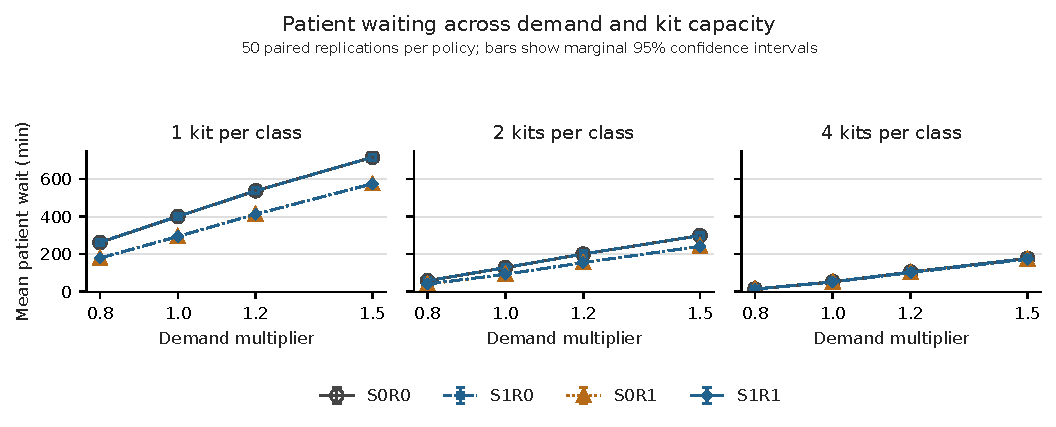
\includegraphics[width=.98\textwidth]{demand_robustness.pdf}
\caption{Mean arrival-to-treatment-start wait across all evaluated conditions. Error bars are marginal 95\% confidence intervals over 50 paired replication blocks. Curves connect evaluated demand settings as visual guides. Near-overlap of S0 and S1 within a dispatch rule reflects the small spacing effects. The common vertical scale preserves the magnitude of severe overload.}
\label{fig:demand}
\end{figure*}

\subsection{Exploratory Capacity and Bypass Checks}
After the primary evaluation, we reused all 6,000 saved cohort-day inputs with uniform spacing. Four two-kit rules used bypass bounds of zero (FCFS), one, two, and effectively unlimited. Two additional rules compared FCFS and bound two with 50 kits per class. The 36,000 runs include 12,000 repeated primary cases, all of which reproduced. These diagnostics are separate from the primary protocol and are reported as exploratory. Patient disadvantage is the fraction of the same patients who wait longer than under two-kit FCFS. We average daily fractions and daily maximum waits within the same 50 blocks. The diagnostics also record total resource workload and periods of queue blocking.

\subsection{Verification and Reproducibility}
Following Sargent \cite{sargent2013}, we separate implementation verification from operational and data validity. Eleven automated tests check single-patient timing, resource integrals, drainage beyond minute 720, scheduling information restrictions, matched inputs, deterministic replay, dispatch activation, the bypass bound, no-show-only days, and resource conservation under stress. An abundant-resource negative control with 50 kits per class gives identical waiting and overtime under R0 and R1, as expected when kit availability cannot block the queue.

Every evaluation run also checks that attendees complete care, kits return, resource occupancy stays within capacity, and patient timestamps remain ordered. All 72,000 runs passed. Paired alternatives contain the same attendees. These checks establish internal consistency; clinical validity still requires comparison with real clinic outcomes.

\section{Results}
\subsection{Reference Condition}
The reference condition has 28 requests per day and two kits per class. Table~\ref{tab:reference} reports means and SDs. Every policy eventually completes the same average of 24.44 attending patients. This setting stresses dentist capacity: mean dentist work is 974.65 minutes against 960 opening-hours dentist-minutes. That ratio is workload divided by available opening time, not observed utilization. Matched policies have the same staff workload, so the comparison holds workload fixed.



With uniform spacing, R1 reduces mean waiting by 34.99 minutes (95\% CI $[-35.90,-34.07]$) relative to S0R0. Spacing alone changes waiting by $+0.40$ minutes (CI $[0.11,0.70]$), a small increase. The combined policy has 92.99 minutes of mean waiting, almost the same as dispatch alone at 92.96 minutes. Its difference from baseline is $-34.96$ minutes (CI $[-35.85,-34.07]$), a descriptive 27.32\% reduction. In this condition, combining spacing with dispatch adds little beyond dispatch.

The factorial waiting effects are $+0.22$ minutes for S (CI $[-0.02,0.45]$) and $-35.17$ for R (CI $[-36.06,-34.28]$). The interaction is $-0.37$ minutes (CI $[-0.67,-0.07]$). Its interval excludes zero, but the effect is small beside the dispatch effect. The combined policy reduces discharge overtime by 48.46 minutes (CI $[-50.63,-46.29]$), yet the last departure still occurs 208.75 minutes after closing on average. A lower value does not make the schedule workable.

\subsection{Demand and Instrument Capacity}
Figure~\ref{fig:demand} shows all policy means. At reference demand, increasing kits from two to four per class changes the R main effect from $-35.17$ minutes to $-1.47$ (CI $[-1.64,-1.30]$). With one kit per class, the effect is $-106.44$ minutes (CI $[-108.57,-104.32]$). In this model, feasible-patient dispatch matters most when kits are scarce.

With 50 kits per class, reference waiting is 50.36 minutes and discharge overtime is 93.55 minutes under either dispatch rule. Removing kit blockage therefore leaves substantial delay. At lower demand (22 requests), dentist workload is 79.5\% of opening capacity, yet dispatch reduces two-kit waiting from 58.03 to 40.79 minutes (paired CI $[-17.94,-16.55]$). The effect is not limited to the reference workload. With abundant kits, lower-demand waiting is 13.45 minutes.





At $1.5\times$ demand with two kits per class, combined-policy waiting is 241.70 minutes and discharge overtime is 524.12 minutes. With four kits per class, the same demand still produces 172.98 minutes of waiting and 346.26 minutes of overtime. At $0.8\times$ demand with four kits, mean waiting is 14.20 minutes under S0R0 and 13.89 under S1R1, leaving little room for improvement. Across all 12 conditions, the absolute S main effect stays below 0.4 minutes. This result applies to the specified proportional-spacing rule, not to appointment optimization in general.

\subsection{Mechanism and Distribution Across Procedures}
At the reference condition, dispatch increases opening-hours dentist occupancy from 66.2\% to 75.1\%. Mean waiting without the patient's own kit changes from 62.30 to 60.57 minutes. Alongside the lower total wait, this pattern is consistent with less queue obstruction while other kits and staff are available. The own-kit measure overlaps other waits and should not be read as an additive breakdown of delay.

Queue histories provide the same explanation. The daily interval in which the first patient lacks a kit, all other treatment resources are free, and a later patient has a ready kit falls from 137.86 to 37.59 minutes under dispatch. The remaining interval reflects the bypass bound. These are queue-state measures, not an additive causal decomposition of patient waiting.

At the reference condition, the combined policy lowers procedure-specific mean waits by 15.38 minutes for routine, 58.83 for restorative, 71.67 for impression, and 67.97 for complex appointments. These averages use only days containing the relevant class. All four paired intervals exclude zero, but the effects differ by class. Daily P90 waiting falls from 234.84 to 192.98 minutes and remains high. A two-bypass limit does not guarantee short waits or fair service.

\subsection{Bypass Limit and Patient Tradeoff}
Table~\ref{tab:fairness} compares the bypass bounds. With bound two, 16.9\% of patients wait longer than under FCFS on average (95\% CI $[16.1,17.8]$), even though the overall mean is lower. Unlimited bypass lowers the mean further, slightly raises the average daily maximum relative to bound two, and disadvantages more patients. The chosen bound is neither optimized nor uniformly fair.

\begin{table}[t]
\caption{Exploratory Bypass Comparison: Reference Demand, Two Kits per Class, Uniform Spacing}
\label{tab:fairness}
\centering\footnotesize
\begin{tabular}{@{}lrrr@{}}
\toprule
Bound & Mean wait & Daily max. wait & Worse than FCFS \\
 & (min) & (min) & (\% of patients) \\
\midrule
0 (FCFS) & 127.94 & 266.77 & 0.0 \\
1 & 103.70 & 239.54 & 14.3 \\
2 & 92.96 & 232.24 & 16.9 \\
Unlimited & 85.28 & 235.44 & 19.7 \\
\bottomrule
\end{tabular}
\end{table}

\section{Operational Implications and Limitations}
The results point to three operating conditions. A blocked first patient can hold the queue even when another kit is ready, and selecting the feasible patient can reduce that delay. When kits are plentiful, the rule adds little. When demand is high, neither rule prevents long waits or overtime. The improvement comes from changing patient order, not from the spacing rule, and coordination cannot replace capacity.

The dispatch rule needs the registered queue, each patient's kit class, available chairs and staff, clean-kit counts, and previous bypasses. A future clinic system would need those fields. A site assessment should measure how often the first patient is kit-blocked, whether staff already choose ready patients, and whether workload fits opening hours. Those observations are still missing.

Several limitations restrict interpretation. First, all input distributions, kit classes, initial stocks, and processing assumptions are synthetic. The reference demand is a comparison setting, not a calibrated normal clinic. In the most constrained cases, draining the system extends far beyond a practical working day. These runs show workload incompatibility in a terminating model; an operating clinic would need cancellations, carryover, or more capacity.

Second, the baseline is strict FCFS by registration. Clinics that already select feasible patients could see a smaller additional benefit. R1 assumes an accurate current resource state and omits observation delays, missing events, and implementation costs. The study does not test whether sensing infrastructure would provide that information. The class-specific kit abstraction and equal counts per class also need clinical review. Because procedure probabilities differ substantially (0.52, 0.28, 0.13, and 0.07) while each class receives the same number of kits, the design isolates class-specific scarcity but does not represent demand-proportional inventory. Equal counts can make common classes appear more constrained and rare classes less constrained than they would be under an inventory policy matched to case mix; results may change with class-specific stock levels and replenishment rules.

Third, the primary experiment uses one bypass limit, and the supplementary bounds do not identify an optimal policy. The weak spacing effect does not show that duration-aware scheduling is generally inferior. Immediate-start sterilizer batches are often underfilled: reference FCFS uses 615.50 total sterilizer-minutes per day. Alternative batching rules would change this workload, including the part that occurs after closing. The experiment also omits provider specialization, breaks, emergencies, alternative duration distributions, and detailed instrument bills of materials. Each independent day starts with a recovered system.

Fourth, the confidence intervals describe numerical variability under fixed assumptions; they do not establish clinical validity. Procedure-level improvements and a bypass bound do not establish equitable service. Calibration would require arrival, treatment, turnover, instrument-circulation, and staffing traces, followed by comparison with current dispatch behavior and other resource-aware policies. Field evaluation would be required before deployment.

\section{Conclusion}
DentDES evaluates two clinic decisions: how to space appointments and which ready patient to treat next. With matched inputs and complete end-of-day accounting, feasible-patient dispatch explains most of the waiting reduction in constrained cases, while the tested spacing rule adds little. More kits reduce the dispatch effect, and overtime remains a separate capacity problem. The model should next be compared with observed patient flow and instrument circulation before anyone tests it in a clinic.

\begin{samepage}
\section*{Data and Code Availability}
The synthetic data and supporting source code for this study are available through a private anonymous reviewer link: https://figshare.com/s/5b71e946fc1346497cea. No patient or other human-subject data were used. Following acceptance, the final artifact will be made publicly available with a persistent DOI.
\end{samepage}

\enlargethispage{1pt}
\begin{thebibliography}{00}
\bibitem{atalan2023} A. Atalan and A. Keskin, ``Estimation of the utilization rates of the resources of a dental clinic by simulation,'' \textit{Sigma Journal of Engineering and Natural Sciences}, vol. 41, no. 2, pp. 423--432, 2023, doi: 10.14744/sigma.2023.00045.
\bibitem{chang2018} W.-J. Chang and Y.-H. Chang, ``Design of a patient-centered appointment scheduling with artificial neural network and discrete event simulation,'' \textit{Journal of Service Science and Management}, vol. 11, no. 1, pp. 71--82, 2018, doi: 10.4236/jssm.2018.111007.
\bibitem{gunal2010} M. M. G\"unal and M. Pidd, ``Discrete event simulation for performance modelling in health care: A review of the literature,'' \textit{Journal of Simulation}, vol. 4, no. 1, pp. 42--51, 2010, doi: 10.1057/jos.2009.25.
\bibitem{vazquez2021} J. I. V\'azquez-Serrano, R. E. Peimbert-Garc\'ia, and L. E. C\'ardenas-Barr\'on, ``Discrete-event simulation modeling in healthcare: A comprehensive review,'' \textit{International Journal of Environmental Research and Public Health}, vol. 18, no. 22, Art. no. 12262, 2021, doi: 10.3390/ijerph182212262.
\bibitem{cayirli2003} T. Cayirli and E. Veral, ``Outpatient scheduling in health care: A review of literature,'' \textit{Production and Operations Management}, vol. 12, no. 4, pp. 519--549, 2003, doi: 10.1111/j.1937-5956.2003.tb00218.x.
\bibitem{gupta2008} D. Gupta and B. T. Denton, ``Appointment scheduling in health care: Challenges and opportunities,'' \textit{IIE Transactions}, vol. 40, no. 9, pp. 800--819, 2008, doi: 10.1080/07408170802165880.
\bibitem{kamali2022} A. H. Kamali, M. Moradi, F. Goodarzian, and P. Ghasemi, ``A discrete event simulation method for performance analysis of an additive manufacturing in the dental clinic,'' \textit{The International Journal of Advanced Manufacturing Technology}, vol. 118, pp. 2949--2979, 2022, doi: 10.1007/s00170-021-08135-7.
\bibitem{gul2011} S. Gul, B. T. Denton, J. W. Fowler, and T. Huschka, ``Bi-criteria scheduling of surgical services for an outpatient procedure center,'' \textit{Production and Operations Management}, vol. 20, no. 3, pp. 406--417, 2011, doi: 10.1111/j.1937-5956.2011.01232.x.
\bibitem{dimascolo2013} M. Di Mascolo and A. Gouin, ``A generic simulation model to assess the performance of sterilization services in health establishments,'' \textit{Health Care Management Science}, vol. 16, no. 1, pp. 45--61, 2013, doi: 10.1007/s10729-012-9210-2.
\bibitem{cardoen2010} B. Cardoen, E. Demeulemeester, and J. Beli\"en, ``Operating room planning and scheduling: A literature review,'' \textit{European Journal of Operational Research}, vol. 201, no. 3, pp. 921--932, 2010, doi: 10.1016/j.ejor.2009.04.011.
\bibitem{guerriero2011} F. Guerriero and R. Guido, ``Operational research in the management of the operating theatre: A survey,'' \textit{Health Care Management Science}, vol. 14, no. 1, pp. 89--114, 2011, doi: 10.1007/s10729-010-9143-6.
\bibitem{harris2024} S. Harris, V. Nino, and D. Claudio, ``Simulating a sterilization processing department to evaluate block schedules and tray configurations,'' \textit{Systems Engineering}, vol. 27, no. 1, pp. 54--73, 2024, doi: 10.1002/sys.21707.
\bibitem{bos2026} H. Bos, G. Hosteins, W. Wijnholds, A. Braaksma, and G. Leeftink, ``Optimization of tray inventory levels in hospitals from an integral perspective,'' \textit{Health Care Management Science}, vol. 29, Art. no. 7, 2026, doi: 10.1007/s10729-025-09743-5.
\bibitem{patrick2008} J. Patrick, M. L. Puterman, and M. Queyranne, ``Dynamic multipriority patient scheduling for a diagnostic resource,'' \textit{Operations Research}, vol. 56, no. 6, pp. 1507--1525, 2008, doi: 10.1287/opre.1080.0590.
\bibitem{armony2015} M. Armony, S. Israelit, A. Mandelbaum, Y. N. Marmor, Y. Tseytlin, and G. B. Yom-Tov, ``On patient flow in hospitals: A data-based queueing-science perspective,'' \textit{Stochastic Systems}, vol. 5, no. 1, pp. 146--194, 2015, doi: 10.1287/14-SSY153.
\bibitem{appuhamilage2025} G. D. K. Kuruppu Appuhamilage, M. Hussain, M. Zaman, and W. A. Khan, ``A health digital twin framework for discrete event simulation based optimised critical care workflows,'' \textit{npj Digital Medicine}, vol. 8, Art. no. 376, 2025, doi: 10.1038/s41746-025-01738-4.
\bibitem{kranzfelder2013} M. Kranzfelder, A. Schneider, A. Fiolka, E. Schwan, S. Gillen, D. Wilhelm, R. Schirren, S. Reiser, B. Jensen, and H. Feussner, ``Real-time instrument detection in minimally invasive surgery using radiofrequency identification technology,'' \textit{Journal of Surgical Research}, vol. 185, no. 2, pp. 704--710, 2013, doi: 10.1016/j.jss.2013.06.022.
\bibitem{hill2022} I. Hill, L. Olivere, J. Helmkamp, E. Le, W. Hill, J. Wahlstedt, P. Khoury, J. Gloria, M. J. Richard, L. H. Rosenberger, and P. J. Codd, ``Measuring intraoperative surgical instrument use with radio-frequency identification,'' \textit{JAMIA Open}, vol. 5, no. 1, Art. no. ooac003, 2022, doi: 10.1093/jamiaopen/ooac003.
\bibitem{zhang2020} X. Zhang, S. K. Lhachimi, and W. H. Rogowski, ``Reporting quality of discrete event simulations in healthcare: Results from a generic reporting checklist,'' \textit{Value in Health}, vol. 23, no. 4, pp. 506--514, 2020, doi: 10.1016/j.jval.2020.01.005.
\bibitem{simpy} SimPy Team, ``Overview,'' \textit{SimPy 4.1.2 documentation}. [Online]. Available: \url{https://simpy.readthedocs.io/en/stable/}. Accessed: Sep. 5, 2026.
\bibitem{cdc} Centers for Disease Control and Prevention, ``Best practices for sterilization monitoring in dental settings,'' May 15, 2024. [Online]. Available: \url{https://www.cdc.gov/dental-infection-control/hcp/dental-ipc-faqs/sterilization-monitoring.html}. Accessed: Sep. 5, 2026.
\bibitem{sargent2013} R. G. Sargent, ``Verification and validation of simulation models,'' \textit{Journal of Simulation}, vol. 7, no. 1, pp. 12--24, 2013, doi: 10.1057/jos.2012.20.
\end{thebibliography}
\end{document}
